% Options for packages loaded elsewhere
\PassOptionsToPackage{unicode}{hyperref}
\PassOptionsToPackage{hyphens}{url}
%
\documentclass[
  12pt,
]{article}
\usepackage{lmodern}
\usepackage{setspace}
\usepackage{amssymb,amsmath}
\usepackage{ifxetex,ifluatex}
\ifnum 0\ifxetex 1\fi\ifluatex 1\fi=0 % if pdftex
  \usepackage[T1]{fontenc}
  \usepackage[utf8]{inputenc}
  \usepackage{textcomp} % provide euro and other symbols
\else % if luatex or xetex
  \usepackage{unicode-math}
  \defaultfontfeatures{Scale=MatchLowercase}
  \defaultfontfeatures[\rmfamily]{Ligatures=TeX,Scale=1}
\fi
% Use upquote if available, for straight quotes in verbatim environments
\IfFileExists{upquote.sty}{\usepackage{upquote}}{}
\IfFileExists{microtype.sty}{% use microtype if available
  \usepackage[]{microtype}
  \UseMicrotypeSet[protrusion]{basicmath} % disable protrusion for tt fonts
}{}
\makeatletter
\@ifundefined{KOMAClassName}{% if non-KOMA class
  \IfFileExists{parskip.sty}{%
    \usepackage{parskip}
  }{% else
    \setlength{\parindent}{0pt}
    \setlength{\parskip}{6pt plus 2pt minus 1pt}}
}{% if KOMA class
  \KOMAoptions{parskip=half}}
\makeatother
\usepackage{xcolor}
\IfFileExists{xurl.sty}{\usepackage{xurl}}{} % add URL line breaks if available
\IfFileExists{bookmark.sty}{\usepackage{bookmark}}{\usepackage{hyperref}}
\hypersetup{
  pdftitle={super-fx},
  pdfauthor={Garner, KG., Knott, Z., Nydam, A., Nolan, CR., Bowman, H., \& Dux, PE.,},
  hidelinks,
  pdfcreator={LaTeX via pandoc}}
\urlstyle{same} % disable monospaced font for URLs
\usepackage[margin=1in]{geometry}
\usepackage{longtable,booktabs}
% Correct order of tables after \paragraph or \subparagraph
\usepackage{etoolbox}
\makeatletter
\patchcmd\longtable{\par}{\if@noskipsec\mbox{}\fi\par}{}{}
\makeatother
% Allow footnotes in longtable head/foot
\IfFileExists{footnotehyper.sty}{\usepackage{footnotehyper}}{\usepackage{footnote}}
\makesavenoteenv{longtable}
\usepackage{graphicx}
\makeatletter
\def\maxwidth{\ifdim\Gin@nat@width>\linewidth\linewidth\else\Gin@nat@width\fi}
\def\maxheight{\ifdim\Gin@nat@height>\textheight\textheight\else\Gin@nat@height\fi}
\makeatother
% Scale images if necessary, so that they will not overflow the page
% margins by default, and it is still possible to overwrite the defaults
% using explicit options in \includegraphics[width, height, ...]{}
\setkeys{Gin}{width=\maxwidth,height=\maxheight,keepaspectratio}
% Set default figure placement to htbp
\makeatletter
\def\fps@figure{htbp}
\makeatother
% Make links footnotes instead of hotlinks:
\DeclareRobustCommand{\href}[2]{#2\footnote{\url{#1}}}
\setlength{\emergencystretch}{3em} % prevent overfull lines
\providecommand{\tightlist}{%
  \setlength{\itemsep}{0pt}\setlength{\parskip}{0pt}}
\setcounter{secnumdepth}{-\maxdimen} % remove section numbering

\usepackage{booktabs}
\usepackage{longtable}
\usepackage{array}
\usepackage{multirow}
\usepackage{wrapfig}
\usepackage{float}
\usepackage{colortbl}
\usepackage{pdflscape}
\usepackage{tabu}
\usepackage{threeparttable}
\usepackage{threeparttablex}
\usepackage[normalem]{ulem}
\usepackage{makecell}
\usepackage{xcolor}
\ifluatex
  \usepackage{selnolig}  % disable illegal ligatures
\fi
\newlength{\cslhangindent}
\setlength{\cslhangindent}{1.5em}
\newenvironment{cslreferences}%
  {\setlength{\parindent}{0pt}%
  \everypar{\setlength{\hangindent}{\cslhangindent}}\ignorespaces}%
  {\par}

\title{super-fx}
\author{Garner, KG., Knott, Z., Nydam, A., Nolan, CR., Bowman, H., \& Dux, PE.,}
\date{2021-04-26 15:49:53}

\begin{document}
\maketitle

% align only at left, not at right.
\iraggedright

\setstretch{1.5}
\textbf{Running headline}: Quantifying effect sizes in cognitive psychology

\textbf{Abstract}:

\clearpage

\hypertarget{introduction}{%
\section{Introduction}\label{introduction}}

\hypertarget{methods}{%
\section{Methods}\label{methods}}

\hypertarget{participants}{%
\subsubsection{Participants}\label{participants}}

The current study utilises a dataset collected in the lab for a previous \href{https://osf.io/nxysg}{pre-registered} project examining the relationship between executive function and individual differences. This dataset consists of performance measures from 313 participants. Participants were undergraduate students, aged 18 to 35 years old (mean = 20.14 yrs, sd = 3.46). Of the total sample, 208 reported being of female sex, and 269 reported being right handed. Participants received course credits as compensation. All procedures were approved by the University of Queensland Human Reseach Ethics Committee and adhered to the \href{https://www.nhmrc.gov.au/about-us/publications/national-statement-ethical-conduct-human-research-2007-updated-2018}{National Statement on Ethical Conduct in Human Research}.

\hypertarget{apparatus}{%
\subsubsection{Apparatus}\label{apparatus}}

Experimental procedures were run on an Apple Mac Minicomputer (OS X Late 2014, 2.8 GHz Intel Core i5) with custom code using the Psychophysics toolbox (v3.0.14)\footnote{Brainard, ``The Psychophysics Toolbox''; Pelli, ``The VideoToolbox Software for Visual Psychophysics.''} in Matlab v2015b. Participants completed 5 tasks; Attentional Blink (AB), Dual Task (DT), Contextual Cueing (CC), Serial Response Task (SRT), and Visual Statistical Learning (VSL). Task order was randomised for each participant, apart from the VSL task, which was presented last. This was because the recognition component of the task may have allowed participants to infer that other tasks were also assessing implicit learning.

\hypertarget{procedures}{%
\subsubsection{Procedures}\label{procedures}}

Across all tasks, participants sat approximately 57 cm from the monitor. An overview of the task procedures is presented in Figure xxxx. Further details regarding the task protocols are presented within each section below. In the interest of reducing working memory load, we provide an overview of the simulation procedures, before detailing the specific procedural and statistical methods for each task.

\begin{figure}

{\centering 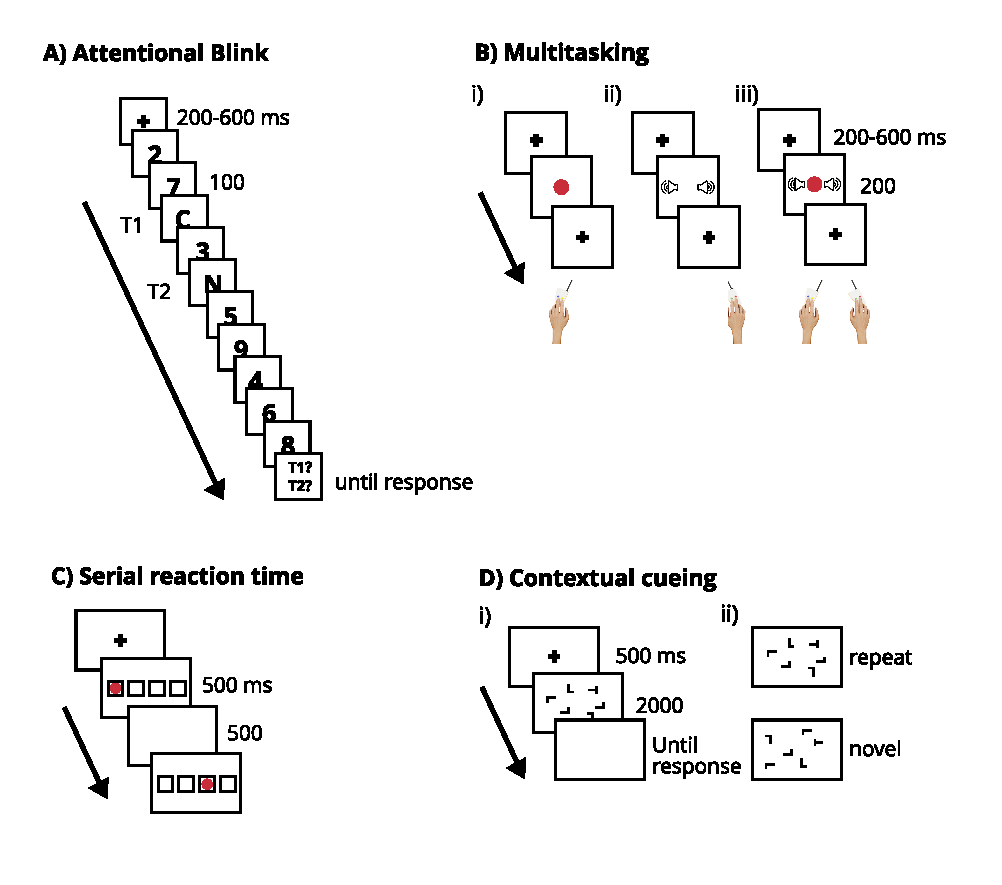
\includegraphics[width=600pix]{/Users/kels/Dropbox/documents/MC-Docs/Super-Effects/images/FigXXXX_alltasks} 

}

\caption{Figure xxxx: Task battery. A) Attentional Blink Paradigm (AB). Participants report the two letter targets from the rapid serial visual presentation of numbers and letters, B) Multitasking Paradigm (MT). Participants make a discriminate the colour of a disc, a complex tone, or both C) Contextual Cueing Paradigm (CC). i) Participants perform an inefficient visual search task. ii) Unknown to participants, half of the search arrays are repeated throughout the course of the experiment. D) Serial reaction time task (SRT). Participants respond to one of four stimuli, each mapped to a spatially-compatible button press. Unknown to participants, for half of the blocks the stimulus follows a repeating sequence. E) Visual Statistical Learning Paradigm (VSL): i) 12 shapes are grouped into 6 base pairs. ii) Learning: three of the six pairs are presented as an array, this is repeated as participants passively view the displays. iii) Test: participants are presented with a base pair, and a novel pair formed from a recombination of the 12 shapes, and is asked which of the two pairs they have seen previously.}\label{fig:paradigm}
\end{figure}

All the \href{}{data} and \href{https://github.com/kel-github/Super-Effects}{code} used for the current analysis are available online. To ascertain that we attained the typically observed findings for each of the paradigms under study, we first applied the conventional statistical model for that paradigm on the full dataset (N=313), the details of which are presented below in the context of each task. Next we implemented a simulation procedure to determine the effect size and p-values that would be attained over \(k\) experiments across multiple sample sizes.

\hypertarget{sampling-procedure}{%
\paragraph{Sampling procedure}\label{sampling-procedure}}

To simulate \(k\) experiments at our chosen sample sizes (N), we developed a sampling procedure that sought to balance the potentially increasing homegeneity of samples as N approached our largest possible sample size (N=313) against the heterogeneity of information offered by the whole dataset. Specifically, it could be that as N approaches 313, the overlap of participants between subsamples may be greater than when N equals a much lower number; e.g.~13. It could then be that decreasing variability in effect size estimates across \(k\) is due to the decrease in variability of the subsamples, rather than an increase in precision that would be expected with a larger N. Therefore at each level of N, we first selected a subsample from the total dataset \emph{without} replacement. From this subsample, we further subsampled \(k\) = 1000 samples of the given N \emph{with} replacement. The relevant analysis was then applied to each of these subsamples. This latter sampling with replacement ensured that the data upon which the analysis was performed carried the Markov property. However, given at lower Ns this could result in a significant loss of information (for example, conclusions regarding the distributions of effect sizes for lower N samples would be based solely on a dataset comprising that lower N (e.g.~N=13), and therefore, may lose critical information, we repeated this process over \(j\) = 1000 iterations. Therefore each density at each N reflects 1000\^{}1000 simulated experiments. We refer to this now as the two-step sampling procedure: \(j\) = 1000, \(k\) = 1000. It is worth noting that we compared this procedure to a simpler one where we performed the two-step sampling procedure with \(j\) = 1 (i.e.~we only sampled N without replacement once), and to a one-step sampling procedure where we sampled N with replacement from the entire dataset (therefore we did not correct against potentially increasing homogeneity of the sample, although note that the Markov property is retained in this sampling procedure), therefore \(k\)=1000 and \(j\) = 0. Outcomes were highly comparable between the sampling procedures, with the two-step procedure (\(j\) = 1000) offering better resolution of the resulting densities (see Supplemental Figure XXXX for a representative example). For each task, we sampled across 20 different Ns, defined on a logarithmic interval between N=13 and N=313. We opted for logarithmic interval given the decreasing information gain from increasing N's at higher N values.

\textbackslash begin\{figure\}

\{\centering \includegraphics[width=600pix]{/Users/kels/Dropbox/documents/MC-Docs/Super-Effects/images/SuppFigXXXX_AB_sampling}

\}

\caption{Supplemental Figure xxxx: Comparison between sampling procedures for the AB task data fit with a repeated measures ANOVA for 4 levels of N; densities of observed effect sizes for the A) two-step sampling procedure j=1000^k=1000, the B) two-step sampling procedure, j=1^k=1000, and C) the one-step procedure, $k$ = 1000}

(\#fig:supp\_sampling)
\textbackslash end\{figure\}

Specific details regarding which analyes were applied to each \(k\) sample are detailed below. Given a) the documented advantages of linear mixed effects models (LME) over repeated-measures ANOVA {[}Muth et al.\footnote{``Alternative Models for Small Samples in Psychological Research.''} Bagiella, Sloan, and Heitjan;\footnote{``Mixed-Effects Models in Psychophysiology.''} mccullochRepeatedMeasuresANOVA2005{]}, b) that only a conceptual proxy of \(\eta_{p}^{2}\) is computable from these models,\footnote{Brysbaert and Stevens, ``Power Analysis and Effect Size in Mixed Effects Models.''} and c) there exists no data that we know of that quantifies to what extent we can expect comparable outcomes between both methods, we (where relevant) opted to apply both the standard statistical model, and a LME model to each \(k\) sample. Specific model specifications are detailed below. Note that given the iterative fitting procedure, and therefore the increased temporal duration of fitting that is inherent to the LME approach, the models specified were the simplest possible. The computational requirements for fitting more complex models would have resulted in simulations running for over 11 months. Therefore, the following results should be interpreted with the caveat in mind that a more complex model may well yield different results in the LME case. In the case of the VSL paradigm, we instead apply a prevalence statistic test, which provides an appropriate inferential statistical test when the dependent variable is an information based measure, such as accuracy.\footnote{Allefeld, Görgen, and Haynes, ``Valid Population Inference for Information-Based Imaging.''}

From each set of simulations (per task) we report the following: 1) to assess the best estimate of the effect size of interest and its variability, we report the central tendency and variability of the distribution of effect sizes observed for our highest N (N=313) (apart from in once case of bimodality, where we report \textbf{suggestions for this would be great!}. 2) to determine imprecision in current effect size estimates present in the field, we report the ratio of the 95\% quantiles of the effect size densities observed for the most precise estimate, relative to that oberved for the N that reflects the median sample size in the field. 3) To determine the N required to achieve 90\% power to reject the null hypothesis, we report the N for which over 90\% of p-values pass the threshold for significance (\(\alpha\)=.05). 4) To compare outcomes between the standard and LME approaches, we compare the ratio of 95\% quantiles of the effect sizes observed for each level of N, and 5) whether there is agreement in the N required to achieve greater than 90\% statistical power.

\hypertarget{attentional-blink-ab}{%
\paragraph{Attentional Blink (AB)}\label{attentional-blink-ab}}

\hypertarget{protocol}{%
\subparagraph{Protocol}\label{protocol}}

The AB protocol was the same as that reported in.\footnote{Bender et al., ``On the Relationship Between Response Selection and Response Inhibition.''} Each trial began with a black fixation cross presented in the center of a gray screen {[}RGB: 128, 128, 128{]} for a variable interval of 200-600 ms. On each trial, letters targets and digit distracters were each presented centrally for 100 ms in rapid serial presentation. The eight distractors were drawn without replacement from the digits 2-9. The target letters were randomly selected from the English alphabet, excluding I, L, O, Q, U, V and X. The first target (T1) was the third item to be presented (serial position 3), and T2 was presented at either lag 2 (200 ms), 3 (300 ms), 5 (500 ms) or 7 (700 ms) relative to T1. All stimuli subtended 2.7\(^\circ\) visual angle. Participants were instructed to make an unspeeded report of the identity of both targets at the end of each trial. Participants completed 24 practice trials and four test blocks of 24 trials. For the current analysis we calculated T2 accuracy, given that T1 was correctly reported (T2\textbar T1), for each lag.

\hypertarget{statistical-analysis}{%
\subparagraph{Statistical Analysis}\label{statistical-analysis}}

As is typical for the field, and to ascertain the effectiveness of the lag manipulation, T2\textbar T1 accuracy was subject to a repeated measures ANOVA, with lag (2, 3, 5, \& 7) as the independent variable. This analysis was also applied to each \(k\) sample. For each \(k\) sample, \(\eta_{p}^{2}\) and the resulting \(p\) value were taken for the main effect of lag.

We also applied a LME to estimate the effect of lag, with a random intercept for each participant (\(j\)) and an intercept for random error (\(i\)):

\[y_{ij} \sim lag + e_{i} + e_{ij}\]

The \(\eta_{p}^{2}\) proxy was taken as the ratio of the estimated fixed effect of interest (lag) to the squareroot of the sum of the variance accounted for by the random effects in the model (see\footnote{Brysbaert and Stevens, ``Power Analysis and Effect Size in Mixed Effects Models.''}):

\[\hat{\eta_{p}^{2}} = \frac{lag}{\sqrt{\sum{\sigma_{e_{i}}, \sigma_{e_{ij}}}}}\]

For this and for all subsequent applications of LME models, the \(p\) value for the regressor of interest (i.e.~lag) was attained by applying Wald's chi-square test as implemented using the Anova function from the car package\footnote{Fox and Weisberg, \emph{An R Companion to Applied Regression}.} for R (note: the results were comparable regardless of whether we used Wald's test or whether we performed a log-likelihood test between the model of interest and a null model, which for the current AB case contained only the two random intercept terms \(e_{ij}\) and \(e_{i}\)).

\hypertarget{multitasking-mt}{%
\paragraph{Multitasking (MT)}\label{multitasking-mt}}

\hypertarget{protocol-1}{%
\subparagraph{Protocol}\label{protocol-1}}

The MT protocol was previously reported in.\footnote{Bender et al., ``On the Relationship Between Response Selection and Response Inhibition.''} Each trial began with a black fixation cross presented in the center of a gray screen {[}RGB: 128, 128, 128{]} for a variable interval of 200-600 ms. Next either one of two possible coloured circles {[}red, RGB: 237, 32, 36 or blue, RGB: 44, 71, 151{]} or one of two possible sounds (complex tones taken from\footnote{Dux et al., ``Isolation of a Central Bottleneck of Information Processing with Time-Resolved FMRI.''}), or both (circle and sound) were presented for 200 ms. The coloured circle subtended 1.3\(^\circ\) visual angle. Participants were instructed to respond to all presented tasks by using the appropriate key press {[}`A' or `S' for left hand responses, `J' or `K' for right hand responses, task-hand mapping was counterbalanced across participants{]}. The DT consisted of 4 blocks of 36 trials, with each trial type (ST visual, ST auditory or DT) randomly mixed within blocks. Participants completed the DT task after completing two ST blocks as practice, one for the visual task and one for the auditory task. Mean response times (RTs) to each task modality x condition were taken as the dependent variable of interest.

\hypertarget{statistical-approach}{%
\subparagraph{Statistical Approach}\label{statistical-approach}}

To ascertain the effectiveness of the multitasking manipulation, the data were modelled using a 2 (task-modality: visual-manual vs auditory-manual) x 2 (task: single vs dual) repeated-measures ANOVA. This analysis was also applied to each \(k\) sample; \(\eta_{p}^{2}\) and \(p\) are reported for the main effect of task. We also applied an LME model which included fixed effects regressors for task-modality, task and their interaction, and random intercepts for participants \(e_{ij}\), and measurement error \(e_{i}\). As above, \(\hat{\eta_{p}^{2}}\) was computed as the ratio of the estimated fixed effect for the task regressor to the square root of the summed variance of the estimated random effects. Again, Wald's chi-square test was applied to attain a \(p\) value for the main effect of task.

\hypertarget{contextual-cueing-cc}{%
\paragraph{Contextual Cueing (CC)}\label{contextual-cueing-cc}}

\hypertarget{protocol-2}{%
\subparagraph{Protocol}\label{protocol-2}}

The CC protocol was the same as reported by.\footnote{Nydam, Sewell, and Dux, ``Cathodal Electrical Stimulation of Frontoparietal Cortex Disrupts Statistical Learning of Visual Configural Information.''} Each trial began with a white fixation cross presented on a grey screen {[}RGB: 80, 80, 80. An array of 12 L's and a single T were then presented presented within an invisible 15 x 15 grid that subtended 10\(^\circ\) x 10\(^\circ\) of visual angle. Orientation of each L was determined randomly to be rotated 0\(^\circ\), 90\(^\circ\), 180\(^\circ\) or 270\(^\circ\) clockwise. The T was oriented to either 90\(^\circ\) or 270\(^\circ\). Participants reported whether the T was oriented to the left (using the `z' key) or the right (using the `m' key). The task consisted of 12 blocks of 24 trials. For half the trials in each block, the display was taken (without replacement) from 1 of 12 configurations that was uniquely generated for each participant, where the location of the distractors and target (but not the orientation of the target) was fixed. These trials were called `Repeats'. For the remaining trials, the display was randomly generated for each trial, making them `Novel'. Displays were generated with the constraint that equal items be placed in each quadrant and each eccentricity. Target positions were matched between the repeat and novel displays for both quadrant and eccentricity. The exact location of the item was jittered within each cell for each presentation, to prevent perceptual learning or adaptation to the specific position of the item. The order of display type (repeat vs novel), configuration (1-12) and target orientation (left or right) was randomised for each block. Mean RTs to each block (1:12) and display type (repeat vs novel) were taken as the dependent variable of interest.

\hypertarget{statistical-approach-1}{%
\subparagraph{Statistical Approach}\label{statistical-approach-1}}

To ascertain whether participants speeded responses to repeat relative to novel trials over the course of the experiment (i.e.~whether participants learned the statistical regularities of the repeated arrays), the data were subject to a block (1:12) x condition (repeat vs novel array) repeated measures ANOVA. Specifically, learning should be evidenced by a significant block x condition interaction. This analysis was applied to each \(k\) sample, and we report \(\eta_{p}^{2}\) and \(p\) for the block x condition interaction. We also applied LME models, containing fixed effects regressors for block, condition and their interaction, and random intercepts for subjects and general measurement error. We report \(\hat{\eta_{p}^{2}}\) for the block x condition interaction and the resulting \(p\) value from Wald's chi-square test.

\hypertarget{serial-response-task-srt}{%
\paragraph{Serial Response Task (SRT)}\label{serial-response-task-srt}}

\hypertarget{protocol-3}{%
\subparagraph{Protocol}\label{protocol-3}}

The SRT was adapted from {[}nissenAttentionalRequirementsLearning1987{]}. The task began with a {[}{]}. Four square placeholders were presented across the horizontal meridian, subtending w\(^\circ\) x h\(^\circ\). A red circle {[}RGB: {]} appeared in one of the 4 squares for 500 ms. This served as the target stimulus. Participants responded by pressing the finger of their dominant hand that spatially aligned to the placeholder within which the circle appeared, using the relevant `j', `k', `l' or `;' keys. The next target stimulus would appear 500 ms after the correct response had been made. Participants completed 4 blocks of 100 trials. For blocks 1 and 4, the location of the target stimulus for each trial was randomly selected from a uniform distribution. These blocks are referred to as `Random'. For blocks 2 and 3, a repeating sequence of 10 elements was used to determine the target location. The sequence was repeated 10 times. The repeating sequence was 4-2-3-1-3-2-4-2-3-1, with 1 being the leftmost placeholder, and 4 being the rightmost placeholder. These blocks are referred to as `Repeats'. Of interest is the RT for Random and Repeat blocks in the latter half of the experiment (block 4 vs 3).

\hypertarget{statistical-approach-2}{%
\subparagraph{Statistical Approach}\label{statistical-approach-2}}

To ascertain whether participants learned the repeating sequences, RTs in the final block of repeats (block 3) were compared to those in the final block of random trials (block 4) using a paired-samples t-test. This analysis was also applied to each \(k\) sample, and we present the resulting Cohen's \(d\) and \(p\) value from each test. We also applied an LME approach where we fit models with a fixed effects regressor for block (3 vs 4), and included the same random intercepts as described above. We report the resulting \(\hat{\eta_{p}^{2}}\) and \(p\) values for the fixed effect of block.

\hypertarget{visual-statistical-learning-vsl}{%
\paragraph{Visual Statistical Learning (VSL)}\label{visual-statistical-learning-vsl}}

\hypertarget{protocol-4}{%
\subparagraph{Protocol}\label{protocol-4}}

The VSL task was adapted from Fiser and Aslin {[}-fiserUnsupervisedStatisticalLearning2001{]}. For each participant, twelve abstract shapes were grouped into 6 base pairs. On each trial of the learning phase, three base pairs were randomly positioned onto a 3 x 3 grid, which subtended ?\(^\circ\) of visual angle. Each shape subtended ?\(^\circ\). A total of 144 of these displays were each presented for 2000 ms, interleaved with a blank screen presented for 1000 ms. Participants were instructed to pay attention to the displays. The test phase consisted of trials where two shape pairs were each presented for 2000 ms, with an intervening blank screen lasting 1000 ms. One pair was selected from the 6 base pairs for that participant, and one pair was formed by a novel recombination formed by randomly selecting two of the 12 shapes, with the constraint that a base pair could not be selected. Participants were instructed to report which of the two pairs was more familiar, using the `z' and `m' keys to denote the first or second pair respectively, with the exact mapping counterbalanced across participants. Paticipants completed a total of 24 trials, with each base pair presented 4 times. The order of base and novel pairs was counterbalanced across trials, and trial order was randomised for each participant. Response accuracy in the testing phase was taken as the dependent variable of interest.

\hypertarget{statistical-approach-3}{%
\subparagraph{Statistical Approach}\label{statistical-approach-3}}

To assess whether participants recognised familiar base pairs more than would be expected by chance, it is typical to apply a one sample t-test to recognition test accuracies, against theoretical chance (p=.5) (e.g.~\footnote{Fiser and Aslin, ``Unsupervised Statistical Learning of Higher-Order Spatial Structures from Visual Scenes.''}). Therefore we applied this test to our data to determine if our results corroborated that of the field. We also applied this test to each \(k\) sample, and we report the resulting Cohen's \(d\) and \(p\) values.

Implementing the prevalence statistic typically involves a two step permutation procedure. First, a null distribution is generated for each participant's accuracies (first level permutations), given their responses and the trials to which they were exposed. This is typically attained by shuffling the trial labels over multiple iterations (e.g.~\(m\) = 1000), and taking the participant's accuracy under each permutation (with the constaint that \(m\) = 1 is the neutral permuation).\footnote{Allefeld, Görgen, and Haynes, ``Valid Population Inference for Information-Based Imaging.''} This yields \(m\) accuracies per participant, that would be attained given the null hypothesis was true. Secondly, to attain the second-level null distribution, each participant's first level permutations are sampled \(i\) times, resulting in \(i\) sets of N accuracies as would be expected given the null hypothesis. The proportion of which the minimum of the neutral accuracies is greater than the minimum accuracies across the \(i\) sets second-level null distributions is taken as a measure of the probability that the neutral accuracies are drawn from the null distribution (i.e.~serves as the \(p\) value of the second-level inferential test). However, given that our sampling procedure already entailed 20*(1000\^{}1000) permutations, we opted to instead apply an analytical definition of the first-level null distribution, using the equation:

\[f_{(flvl)} = xxx \]

To generate the second level null distribution, we then sampled each participant's first level distribution \(i\) = 1000 times.

To attain an estimate of the effect size, we can compute the proportion of the population expected to show the effect \(\gamma\), given the observed \(p\) statistic, using the formula defined by Allefeld et al :

\[\gamma = \frac{\alpha^\frac{1}{N} - p^\frac{1}{N}}{1-p^\frac{1}{N}}\]

\hypertarget{results}{%
\subsection*{Results}\label{results}}
\addcontentsline{toc}{subsection}{Results}

\hypertarget{refs}{}
\begin{cslreferences}
\leavevmode\hypertarget{ref-allefeldValidPopulationInference2016}{}%
Allefeld, Carsten, Kai Görgen, and John-Dylan Haynes. ``Valid Population Inference for Information-Based Imaging: From the Second-Level T-Test to Prevalence Inference.'' \emph{NeuroImage} 141 (November 2016): 378--92. \url{https://doi.org/10.1016/j.neuroimage.2016.07.040}.

\leavevmode\hypertarget{ref-bagiellaMixedeffectsModelsPsychophysiology2000}{}%
Bagiella, Emilia, Richard P. Sloan, and Daniel F. Heitjan. ``Mixed-Effects Models in Psychophysiology.'' \emph{Psychophysiology} 37, no. 1 (2000): 13--20. \url{https://doi.org/https://doi.org/10.1111/1469-8986.3710013}\\
\_eprint: https://onlinelibrary.wiley.com/doi/pdf/10.1111/1469-8986.3710013.

\leavevmode\hypertarget{ref-benderRelationshipResponseSelection2016}{}%
Bender, Angela D., Hannah L. Filmer, K. G. Garner, Claire K. Naughtin, and Paul E. Dux. ``On the Relationship Between Response Selection and Response Inhibition: An Individual Differences Approach.'' \emph{Attention, Perception \& Psychophysics} 78, no. 8 (November 2016): 2420--32. \url{https://doi.org/10.3758/s13414-016-1158-8}.

\leavevmode\hypertarget{ref-brainardPsychophysicsToolbox1997}{}%
Brainard, D. H. ``The Psychophysics Toolbox.'' \emph{Spatial Vision} 10, no. 4 (1997): 433--36\\
tex.ids: brainardPsychophysicsToolbox1997a publisher: Brill section: Spatial Vision.

\leavevmode\hypertarget{ref-brysbaertPowerAnalysisEffect2018}{}%
Brysbaert, Marc, and Michaël Stevens. ``Power Analysis and Effect Size in Mixed Effects Models: A Tutorial.'' \emph{Journal of Cognition} 1, no. 1 (January 2018): 9. \url{https://doi.org/10.5334/joc.10}\\
Number: 1 Publisher: Ubiquity Press.

\leavevmode\hypertarget{ref-duxIsolationCentralBottleneck2006}{}%
Dux, Paul E., Jason Ivanoff, Christopher L. Asplund, and René Marois. ``Isolation of a Central Bottleneck of Information Processing with Time-Resolved FMRI.'' \emph{Neuron} 52, no. 6 (December 2006): 1109--20. \url{https://doi.org/10.1016/j.neuron.2006.11.009}.

\leavevmode\hypertarget{ref-fiserUnsupervisedStatisticalLearning2001}{}%
Fiser, József, and Richard N. Aslin. ``Unsupervised Statistical Learning of Higher-Order Spatial Structures from Visual Scenes.'' \emph{Psychological Science} 12, no. 6 (November 2001): 499--504. \url{https://doi.org/10.1111/1467-9280.00392}\\
Publisher: SAGE Publications Inc.

\leavevmode\hypertarget{ref-foxCompanionAppliedRegression2018}{}%
Fox, John, and Sanford Weisberg. \emph{An R Companion to Applied Regression}. SAGE Publications, 2018\\
Google-Books-ID: uPNrDwAAQBAJ.

\leavevmode\hypertarget{ref-muthAlternativeModelsSmall2016}{}%
Muth, Chelsea, Karen L. Bales, Katie Hinde, Nicole Maninger, Sally P. Mendoza, and Emilio Ferrer. ``Alternative Models for Small Samples in Psychological Research: Applying Linear Mixed Effects Models and Generalized Estimating Equations to Repeated Measures Data.'' \emph{Educational and Psychological Measurement} 76, no. 1 (February 2016): 64--87. \url{https://doi.org/10.1177/0013164415580432}\\
Publisher: SAGE Publications Inc.

\leavevmode\hypertarget{ref-nydamCathodalElectricalStimulation2018}{}%
Nydam, Abbey S., David K. Sewell, and Paul E. Dux. ``Cathodal Electrical Stimulation of Frontoparietal Cortex Disrupts Statistical Learning of Visual Configural Information.'' \emph{Cortex} 99 (February 2018): 187--99. \url{https://doi.org/10.1016/j.cortex.2017.11.008}.

\leavevmode\hypertarget{ref-pelliVideoToolboxSoftwareVisual1997}{}%
Pelli, Denis G. ``The VideoToolbox Software for Visual Psychophysics: Transforming Numbers into Movies.'' \emph{Spatial Vision} 10, no. 4 (January 1997): 437--42. \url{https://doi.org/10.1163/156856897X00366}\\
tex.ids: pelliVideoToolboxSoftwareVisual1997a publisher: Brill section: Spatial Vision.
\end{cslreferences}

\end{document}
